%
% Draw colorful diagrams of geometry theorems without words
% Formatted for an A2 poster
%

\documentclass[12pt]{article}
\usepackage[a2paper]{geometry}

\usepackage{bm}
\usepackage{verbatim,url}

\usepackage{tikz}
\usetikzlibrary{positioning,through,
                calc,intersections,arrows.meta,external}

\textwidth=390mm
\textheight=560mm
\topmargin=-10pt
\oddsidemargin=-5mm

\newcommand*{\mth}[1]{\Large$\bm{#1}$}

\begin{document}
\thispagestyle{empty}

\begin{center}
\textbf{\Huge Geometry Without Words}\\
\mbox{}\\
\textbf{\LARGE Moti Ben-Ari}\\
\mbox{}\\
\L{\texttt{http://www.weizmann.ac.il/sci-tea/benari/}}
\end{center}

\bigskip\bigskip

%
% Median of a triangle is half the base
%
\begin{center}
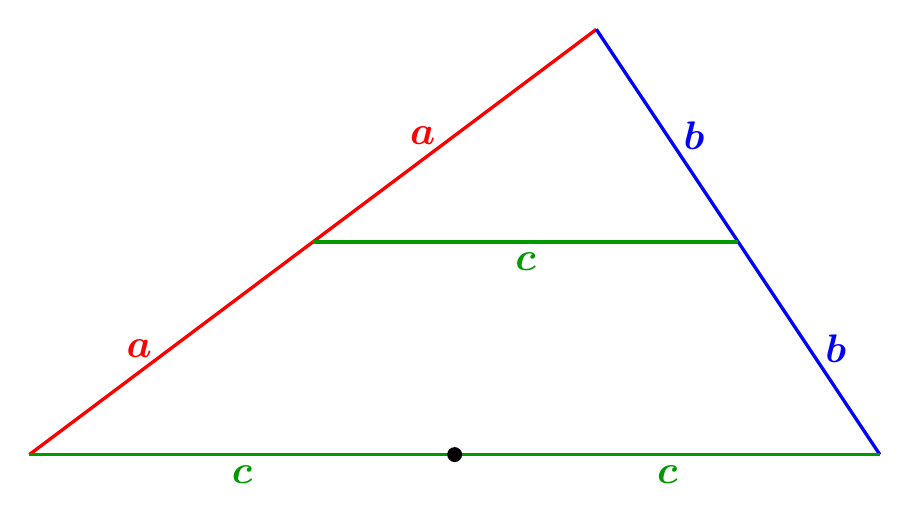
\begin{tikzpicture}[scale=1.8]
% Points of the triangle
\coordinate (a) at (0,0);
\coordinate (b) at (6,0);
\coordinate (c) at (4,3);
% Midpoints of the sides
\coordinate (mid1) at ($(a)!.5!(c)$);
\coordinate (mid2) at ($(b)!.5!(c)$);
% Midpoint of the base
\coordinate (midbase) at ($(a)!.5!(b)$);
% Draw the sides of the triangle: the base is drawn in two parts
\draw[very thick,red] (a) -- node[left,xshift=-3pt] {\mth{a}} (mid1);
\draw[very thick,red] (mid1) -- node[left,xshift=-3pt] {\mth{a}} (c);
\draw[very thick,blue] (b) -- node[right,xshift=2pt] {\mth{b}} (mid2);
\draw[very thick,blue] (mid2) -- node[right,xshift=2pt] {\mth{b}} (c);
% Draw the median
\draw[very thick,green!60!black] (mid1) -- node[below] {\mth{c}} (mid2);
% Draw the base
\draw[very thick,green!60!black] (a) -- node[below] {\mth{c}} (midbase);
\draw[very thick,green!60!black] (b) -- node[below] {\mth{c}} (midbase);
\fill (midbase) circle (1.5pt);
\end{tikzpicture}
%
\hspace{15mm}
%
% Diagonals of parallelogram bisect each other
%
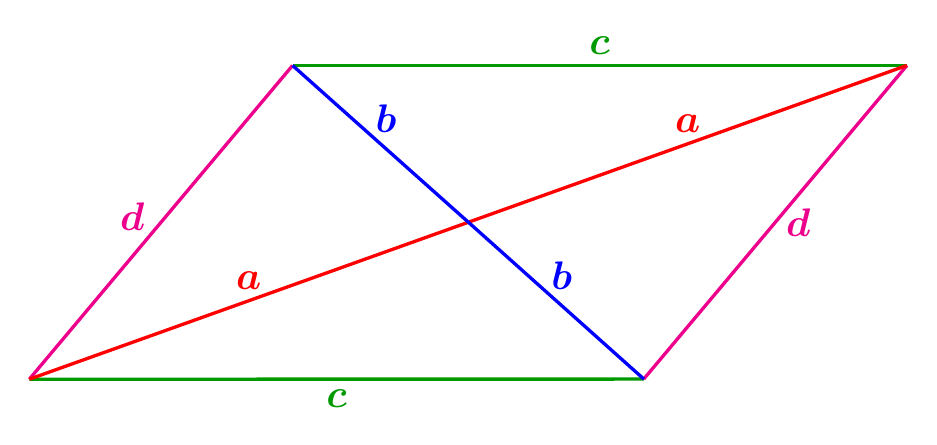
\begin{tikzpicture}[scale=1.3]
% Bottom side of parallelogram
\coordinate (a) at (0,0);
\coordinate (b) at (6,0);
% Draw parallelogram at angle 50
\draw[very thick,magenta] (a) -- node[left,xshift=-2pt,yshift=2pt] {\mth{d}} +(50:4) coordinate (c);
\draw[very thick,green!60!black] (c) -- node[above] {\mth{c}} +(6,0) coordinate (d);
\draw[very thick,magenta] (d) -- node[right] {\mth{d}} +(230:4) coordinate (b);
\draw[very thick,green!60!black] (b) -- node[below] {\mth{c}} (a);
% Name the two diagonals
\path [name path=d1] (a) -- (d);
\path [name path=d2] (b) -- (c);
% Get their intersection
\path [name intersections={of=d1 and d2,by={intersection}}];
% Draw diagonals
\draw[very thick,red] (a) -- node[above] {\mth{a}} (intersection);
\draw[very thick,red] (intersection) -- node[above] {\mth{a}} (d);
\draw[very thick,blue] (b) -- node[above,xshift=2pt] {\mth{b}} (intersection);
\draw[very thick,blue] (intersection) -- node[above,xshift=2pt] {\mth{b}} (c);
\end{tikzpicture}
%
\hspace{15mm}
%
% Diagonals of rhombus bisect each other and are perpendicular
%
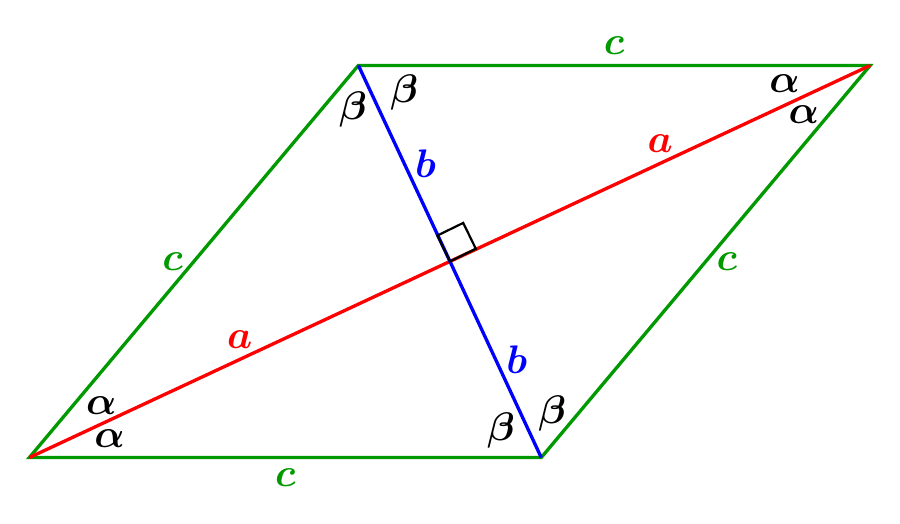
\begin{tikzpicture}[scale=1.3]
% Bottom side of rhombus
\coordinate (a) at (0,0);
\coordinate (b) at (5,0);
% Label angles
\node[above right,xshift=20pt,yshift=0pt] at (a) {\mth{\alpha}};
\node[above right,xshift=17pt,yshift=12pt] at (a) {\mth{\alpha}};
\node[above,xshift=4pt,yshift=6pt] at (b) {\mth{\beta}};
\node[above left,xshift=-6pt,yshift=0pt] at (b) {\mth{\beta}};
% Draw rhombus at angle 50
\draw[very thick,green!60!black] (a) -- node[left] {\mth{c}} ++(50:5) coordinate (c) -- node[above] {\mth{c}} ++(5,0) coordinate (d) -- node[right] {\mth{c}} (b) -- node[below] {\mth{c}} cycle;
% Label angles
\node[below left,xshift=-15pt,yshift=-11pt] at (d) {\mth{\alpha}};
\node[below left,xshift=-22pt,yshift=0pt] at (d) {\mth{\alpha}};
\node[below,xshift=-2pt,yshift=-6pt] at (c) {\mth{\beta}};
\node[below right,xshift=8pt,yshift=0pt] at (c) {\mth{\beta}};
% Name the two diagonals
\path [name path=d1] (a) -- (d);
\path [name path=d2] (b) -- (c);
% Get their intersection
\path [name intersections={of=d1 and d2,by={intersection}}];
% Draw diagonals
\draw[very thick,red] (a) -- node[above] {\mth{a}} (intersection);
\draw[very thick,red] (intersection) -- node[above] {\mth{a}} (d);
\draw[very thick,blue] (b) -- node[right] {\mth{b}} (intersection);
\draw[very thick,blue] (intersection) -- node[right] {\mth{b}} (c);
% Draw square to denote right angle
\draw[thick,rotate=26] (intersection) rectangle +(8pt,8pt);
\end{tikzpicture}
\end{center}

\bigskip\bigskip

%
% Median of a trapezoid is average of sides
%
\begin{center}
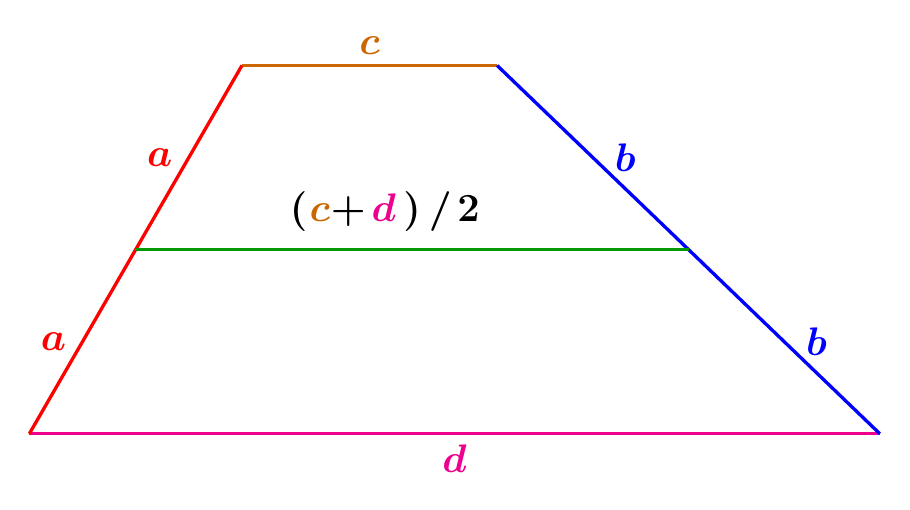
\begin{tikzpicture}[scale=1.8]
% Bottom of trapeze
\coordinate (a) at (0,0);
\coordinate (b) at (6,0);
% Draw the bases of the trapeze
\draw[very thick,magenta] (a) -- node[below] {\mth{d}} (b);
\path (a) -- ++(60:3) coordinate (c) -- ++(1.8,0) coordinate (d);
\draw[very thick,orange!80!black] (c) -- node[above] {\mth{c}} (d);
% Draw the sides of the trapeze in two parts
\coordinate (mid1) at ($(a)!.5!(c)$);
\coordinate (mid2) at ($(b)!.5!(d)$);
\draw[very thick,red] (a) -- node[left,xshift=-2pt] {\mth{a}} (mid1);
\draw[very thick,red] (mid1) -- node[left,xshift=-2pt] {\mth{a}} (c);
\draw[very thick,blue] (b) -- node[right,xshift=4pt] {\mth{b}} (mid2);
\draw[very thick,blue] (mid2) -- node[right,xshift=4pt] {\mth{b}} (d);
% Draw the median
\draw[very thick,green!60!black] (mid1) -- (mid2);
% Display formula in color
\begin{scope}[xshift=19mm,yshift=15mm]
\node[anchor=base] at (0,0) {\mth{(}};
\node[anchor=base,orange!80!black] at (.15,0) {\mth{c}};
\node[anchor=base] at (.35,0) {\mth{+}};
\node[anchor=base,magenta] at (.6,0) {\mth{d}};
\node[anchor=base] at (.8,0) {\mth{)}};
\node[anchor=base] at (1,0) {\mth{/}};
\node[anchor=base] at (1.2,0) {\mth{2}};
\end{scope}
\end{tikzpicture}
%
\hspace{15mm}
%
% Medians of a triangle meet at a point with ratio 1:2
%
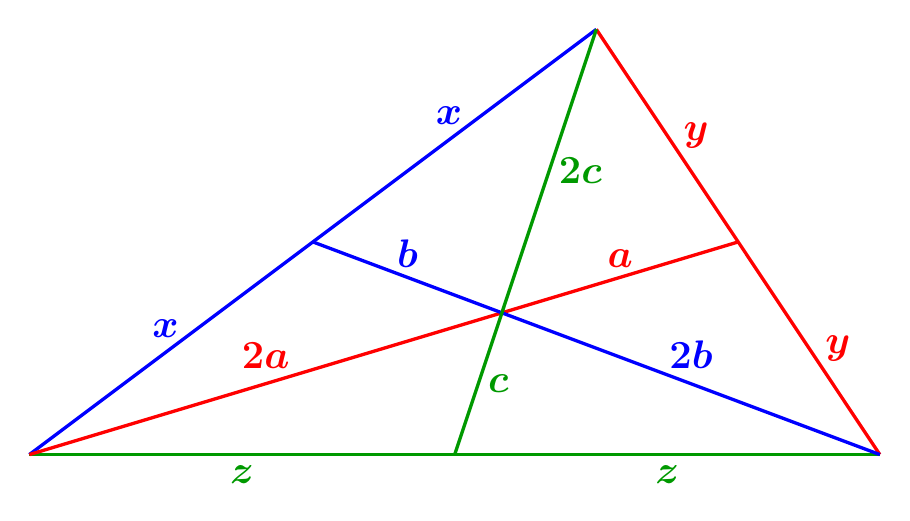
\begin{tikzpicture}[scale=1.8]
\coordinate (a) at (0,0);   % Points of the triangle
\coordinate (b) at (6,0);
\coordinate (c) at (4,3);
% Coordinates of bisectors
\coordinate (ab) at ($(a)!.5!(b)$);
\coordinate (bc) at ($(b)!.5!(c)$);
\coordinate (ac) at ($(a)!.5!(c)$);
% Draw the triangle and bisectors
\draw[blue,very thick] (a) -- node[above,xshift=-2pt] {\mth{x}} (ac) -- node[above,xshift=-2pt] {\mth{x}} (c);
\draw[red,very thick] (b) -- node[right,xshift=2pt] {\mth{y}} (bc) -- node[right,xshift=2pt] {\mth{y}} (c);
\draw[green!60!black,very thick] (a) -- node[below] {\mth{z}} (ab) -- node[below] {\mth{z}} (b);
\draw[very thick,red,name path=da] (a) -- (bc);
\draw[very thick,blue,name path=db] (b) -- (ac);
\draw[very thick,green!60!black,name path=dc] (c) -- (ab);
% Get their intersection
\path [name intersections={of=da and db,by={intersection}}];
% Labels
\path (a) -- node[above,red,yshift=2pt] {\mth{2a}} (intersection);
\path (bc) -- node[above,red] {\mth{a}} (intersection);
\path (b) -- node[above,blue,yshift=2pt] {\mth{2b}} (intersection);
\path (ac) -- node[above,blue] {\mth{b}} (intersection);
\path (c) -- node[right,green!60!black] {\mth{2c}} (intersection);
\path (ab) -- node[right,green!60!black] {\mth{c}} (intersection);
\end{tikzpicture}
%
\hspace{15mm}
%
% Inscribed circle center at meeting of angle bisectors
%
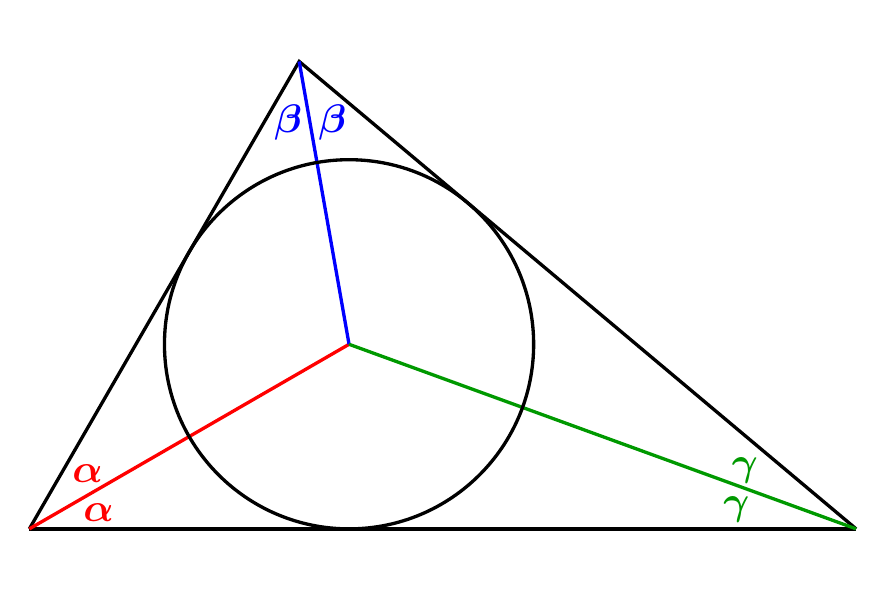
\begin{tikzpicture}[scale=2.1,baseline=-20pt]
% Draw base and path two lines at known angles
\draw[very thick] (0,0) coordinate (a) -- (0:5) coordinate (b);
\path[name path=ac] (a) -- +(60:3.5);
\path[name path=bc] (b) -- +(140:4.5);
% Get their intersection and draw lines to third vertex
\path[name intersections={of=ac and bc,by=c}];
\draw[very thick] (a) -- (c) -- (b);
% Path bisectors of two lines
\path[name path=bia,blue] (a) -- +(30:3.6);
\path[name path=bib,red] (b) -- +(160:5);
% Intersection of angle bisectors
\path [name intersections={of=bia and bib,by=center}];
%% Draw angle bisectors to center
\draw[very thick,red] (a) -- (center);
\draw[very thick,blue] (c) -- (center);
\draw[very thick,green!60!black] (b) -- (center);
%% Labels of angles
\node[red,right,xshift=16pt,yshift=6pt] at (a) {\mth{\alpha}};
\node[red,right,xshift=12pt,yshift=20pt] at (a) {\mth{\alpha}};
\node[blue,below,xshift=-4pt,yshift=-12pt] at (c) {\mth{\beta}};
\node[blue,below,xshift=12pt,yshift=-12pt] at (c) {\mth{\beta}};
\node[green!60!black,left,xshift=-35pt,yshift=7pt] at (b) {\mth{\gamma}};
\node[green!60!black,left,xshift=-32pt,yshift=21pt] at (b) {\mth{\gamma}};
%% Get perpendicular from center to one side and draw circle
\coordinate (perp) at ($(a)!(center)!(b)$);
\node [very thick,draw,circle through=(perp)] at (center) {};
\end{tikzpicture}
\end{center}

\bigskip\bigskip

%
% Perpendicular bisectors meet in the center of the circumscribed circle
%
\begin{center}
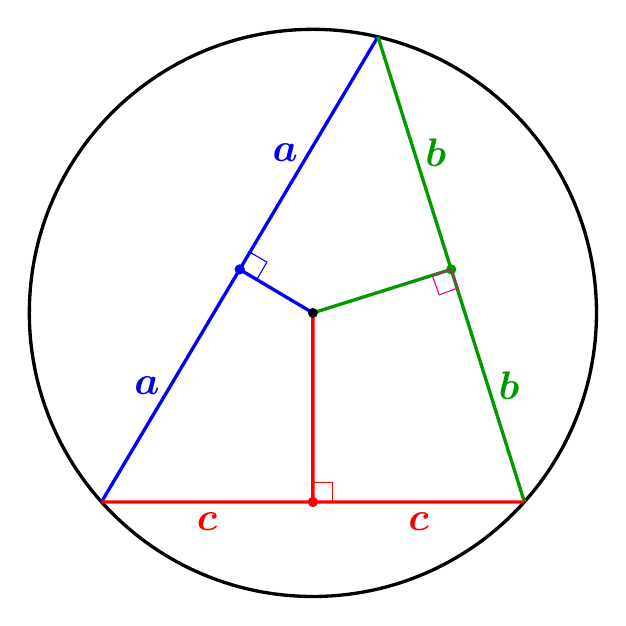
\begin{tikzpicture}[scale=1.2]
% Circle goes from (a) to (b)
\coordinate (a) at (0,0);
\coordinate (b) at (6,0);
% Line containing lower points is (c) -- (d)
\coordinate (c) at (0,-2);
\coordinate (d) at (6,-2);
% Line containing upper points is (e) -- (f)
\coordinate (e) at (0,2);
\coordinate (f) at (4,3);
% Name the two chords
\path [name path=chord1] (c) -- (d);
\path [name path=chord2] (e) -- (f);
% Name the coordinate of the center of the circle
\coordinate (center) at ($ (a)!.5!(b) $);
% Draw a circle whose center is half-way between (a) and (b) through (a)
\node [draw,very thick,circle through=(a),name path=circ] at (center) {};
% Get intersections of the upper and lower lines with the circle
\path [name intersections={of=circ and chord1,by={i1,i2}}];
\path [name intersections={of=circ and chord2,by={i3,i4}}];
% Draw triangle
\draw [very thick,blue] (i1) -- node[left] {\mth{a}} ($(i1)!.5!(i3)$) --
  node[left] {\mth{a}} (i3);
\draw[very thick,green!60!black] (i3) -- node[right] {\mth{b}} ($(i3)!.5!(i2)$) --
  node[right] {\mth{b}} (i2);
\draw[very thick,red] (i2) -- node[below] {\mth{c}} ($(i2)!.5!(i1)$) -- 
  node[below] {\mth{c}} (i1);
% Draw three perpendicular bisectors
\draw [very thick,red,fill] (center) -- ($(i1)!(center)!(i2)$)
  circle[radius=1pt];
\draw [very thick,blue,fill] (center) -- ($(i1)!(center)!(i3)$)
  circle[radius=1pt];
\draw [very thick,green!60!black,fill] (center) -- ($(i2)!(center)!(i3)$)
  circle[radius=1pt];
% Draw squares to denote right angles
\draw[red] ($ (i1) !.5! (i2) $) rectangle +(6pt,6pt);
\draw[blue,rotate=-30] ($ (i1) !.5! (i3) $) rectangle +(6pt,6pt);
\draw[magenta,rotate=-160] ($ (i3) !.5! (i2) $)
  rectangle +(6pt,6pt);
\fill (center) circle (1.5pt);
\end{tikzpicture}
%
\hspace{50mm}
%
% Opposite angles in an inscribed quadrilateral add up to 180
%
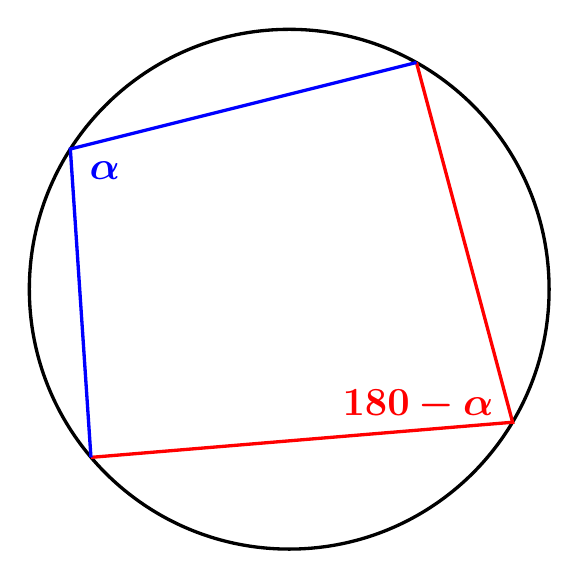
\begin{tikzpicture}[scale=1.1]
% Circle goes from (a) to (b)
\coordinate (a) at (0,0);
\coordinate (b) at (6,0);
% Line containing lower points is (c) -- (d)
\coordinate (c) at (0,-2);
\coordinate (d) at (6,-1.5);
% Line containing upper points is (e) -- (f)
\coordinate (e) at (0,1.5);
\coordinate (f) at (6,3);
% Name the upper and lower lines
\path [name path=chord1] (c) -- (d);
\path [name path=chord2] (e) -- (f);
% Draw a circle whose center is half-way between (a) and (b) through (a)
\node [draw,very thick,circle through=(a),name path=circ] at ($ (a)!.5!(b) $) {};
% Get intersections of the upper and lower lines with the circle
\path [name intersections={of=circ and chord1,by={i1,i2}}];
\path [name intersections={of=circ and chord2,by={i3,i4}}];
% Draw the two subtended angles
\draw[very thick,red] (i1) -- (i2)
  node[left,xshift=-3pt,yshift=6pt] {\mth{180-\alpha}} -- (i3);
\draw[very thick,blue] (i1) -- (i4)
  node[right,xshift=3pt,yshift=-8pt] {\mth{\alpha}} -- (i3);
\end{tikzpicture}
%
\hspace{45mm}
%
% Sums of opposite sides of circumscribed quadrilateral are equal
%
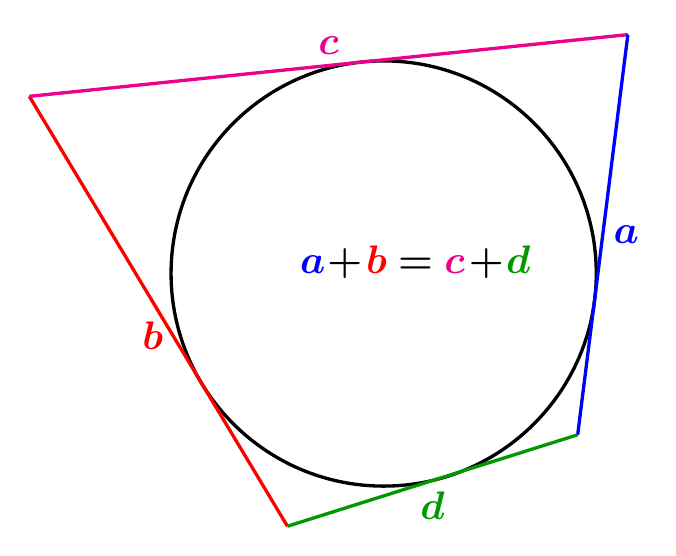
\begin{tikzpicture}[scale=.9]
% Circle goes from (a) to (b)
\coordinate (x) at (0,3);
\coordinate (y) at (6,3);
\coordinate (a) at (-2,5.5);
% Draw a circle whose center is half-way between (a) and (b) through (a)
\node [draw,very thick,circle through=(x),name path=circ] (circle) at ($ (x)!.5!(y) $) {};
% Draw tangent lines
\coordinate (tan1) at (tangent cs:node=circle, point={(a)}, solution=1);
\draw[very thick,red] (a) -- node[below,xshift=-2pt] {\mth{b}}
  ($(a)!1.5!(tan1)$) coordinate (b);
\coordinate (tan2) at (tangent cs:node=circle, point={(a)}, solution=2);
\draw[very thick,magenta] (a) -- node[above] {\mth{c}}
  ($(a)!1.8!(tan2)$) coordinate (c);
\coordinate (tan3) at (tangent cs:node=circle, point={(c)}, solution=2);
\draw[very thick,blue] (c) -- node[right] {\mth{a}}
  ($(c)!1.51!(tan3)$)  coordinate (d);
\draw[very thick,green!60!black] (b) -- node[below] {\mth{d}} (d);
% Display formula in color
\begin{scope}[xshift=2cm,yshift=3cm]
\node[anchor=base,blue] at (0,0) {\mth{a}};
\node[anchor=base] at (.45,0) {\mth{+}};
\node[anchor=base,red] at (.9,0) {\mth{b}};
\node[anchor=base] at (1.45,0) {\mth{=}};
\node[anchor=base,magenta] at (2,0) {\mth{c}};
\node[anchor=base] at (2.45,0) {\mth{+}};
\node[anchor=base,green!60!black] at (2.9,0) {\mth{d}};
\end{scope}
\end{tikzpicture}
\end{center}

\bigskip\bigskip

%
% Angles of tangent and angle subtending a chord are equal
%
\begin{center}
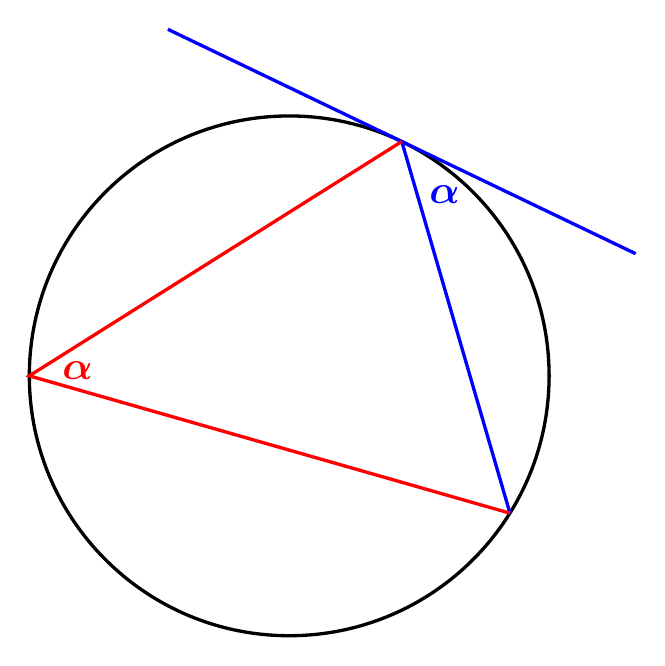
\begin{tikzpicture}[scale=1.1]
% Circle goes from (a) to (b)
\coordinate (a) at (0,0);
\coordinate (b) at (6,0);
% Line containing lower point (d)
\coordinate (d) at (7,-2);
% Point outside circle is (e)
\coordinate (e) at (1.6,4);
% Name the lower chord
\path [name path=chord] (a) -- (d);
% Draw a circle whose center is half-way between (a) and (b) through (a)
\node [draw,very thick,circle through=(a),name path=circ] (circle) at ($ (a)!.5!(b) $) {};
% Get intersection of the lower line with the circle
\path [name intersections={of=circ and chord,by={i1,i2}}];
% Draw the tangent line
\coordinate (tan) at (tangent cs:node=circle, point={(e)}, solution=2);
\draw[very thick,blue] (e) -- ($ (e)!2!(tan) $);
% Draw the triangle
\draw [very thick,blue] (tan) node[below right,xshift=6pt,yshift=-12pt] {\mth{\alpha}} -- (i2);
\draw [very thick,red] (tan) -- (a) node[right,xshift=8pt,yshift=2pt] {\mth{\alpha}} -- (i2);
\end{tikzpicture}
%
\hspace{25mm}
%
% Thale's theorem
%
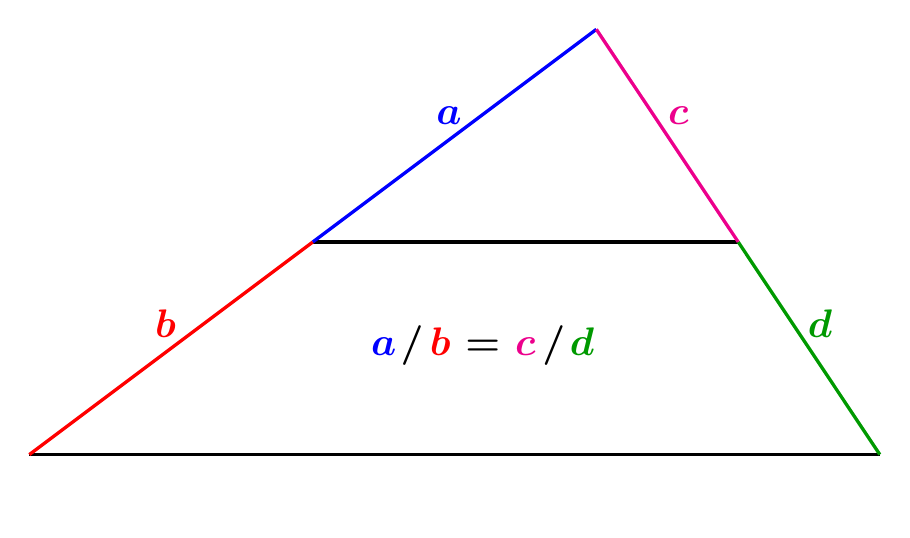
\begin{tikzpicture}[scale=1.8,baseline=-20pt]
% Points of the triangle
\coordinate (a) at (0,0);
\coordinate (b) at (6,0);
\coordinate (c) at (4,3);
% Midpoints of the sides
\coordinate (mid1) at ($(a)!.5!(c)$);
\coordinate (mid2) at ($(b)!.5!(c)$);
% Draw the base and median
\draw[very thick] (a) -- (b);
\draw[very thick] (mid1) -- (mid2);
% Get the median
\coordinate (midbase) at ($(a)!.5!(b)$);
% Draw the triangle, sides in two parts
\draw[very thick,red] (a) -- node[above,xshift=-2pt] {\mth{b}} (mid1);
\draw[very thick,blue] (mid1) -- node[above,xshift=-2pt] {\mth{a}} (c);
\draw[very thick,green!60!black] (b) -- node[above,xshift=4pt] {\mth{d}} (mid2);
\draw[very thick,magenta] (mid2) -- node[above,xshift=4pt] {\mth{c}} (c);
\begin{scope}[xshift=2.5cm,yshift=.7cm]
\node[anchor=base,blue] at (0,0) {\mth{a}};
\node[anchor=base] at (.2,0) {\mth{/}};
\node[anchor=base,red] at (.4,0) {\mth{b}};
\node[anchor=base] at (.7,0) {\mth{=}};
\node[anchor=base,magenta] at (1,0) {\mth{c}};
\node[anchor=base] at (1.2,0) {\mth{/}};
\node[anchor=base,green!60!black] at (1.4,0) {\mth{d}};
\end{scope}
\end{tikzpicture}
%
\hspace{20mm}
%
%  Angle bisector splits side proportionally
%
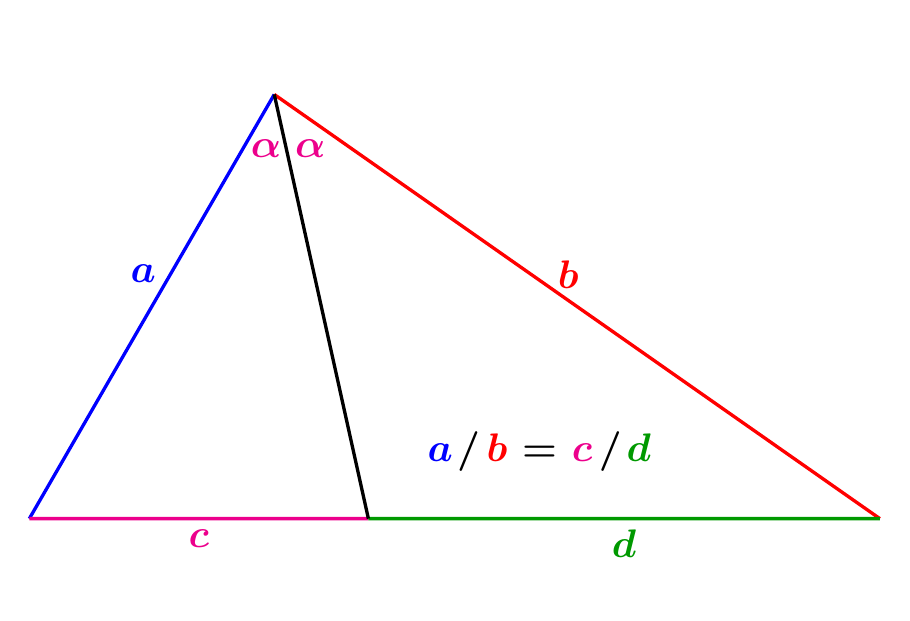
\begin{tikzpicture}[scale=1.8]
% Draw base and path two lines at known angles
\path[name path=ab] (0,0) coordinate (a) -- (0:6) coordinate (b);
\path[name path=ac] (a) -- node[left,xshift=-2pt,blue] {\mth{a}} +(60:4);
\path[name path=bc] (b) -- node[right,xshift=6pt,red] {\mth{b}} +(145:6);
% Get their intersection and draw lines to third vertex
\path[name intersections={of=ac and bc,by=c}];
\draw[blue,very thick] (a) -- (c);
\draw[red,very thick] (c) -- (b);
% Path bisectors of two lines
\path[name path=bisector] (c) -- +(-77.5:3.6);
% Intersection of angle bisectors
\draw[name intersections={of=bisector and ab,by=int}];
% Draw base of triangle
\draw[very thick,magenta] (a) -- node[below] {\mth{c}} (int);
\draw[very thick,green!60!black] (int) -- node[below] {\mth{d}} (b);
% Draw bisector and label angle
\draw[very thick] (c) -- (int);
\node[magenta,below,xshift=-3pt,yshift=-13pt] at (c) {\mth{\alpha}};
\node[magenta,below,xshift=13pt,yshift=-13pt] at (c) {\mth{\alpha}};
% Display formula in color
\begin{scope}[xshift=29mm,yshift=4mm]
\node[anchor=base,blue] at (0,0) {\mth{a}};
\node[anchor=base] at (.2,0) {\mth{/}};
\node[anchor=base,red] at (.4,0) {\mth{b}};
\node[anchor=base] at (.7,0) {\mth{=}};
\node[anchor=base,magenta] at (1,0) {\mth{c}};
\node[anchor=base] at (1.2,0) {\mth{/}};
\node[anchor=base,green!60!black] at (1.4,0) {\mth{d}};
\end{scope}
\end{tikzpicture}
\end{center}

\bigskip\bigskip

%
% Intersecting chords
%
\begin{center}
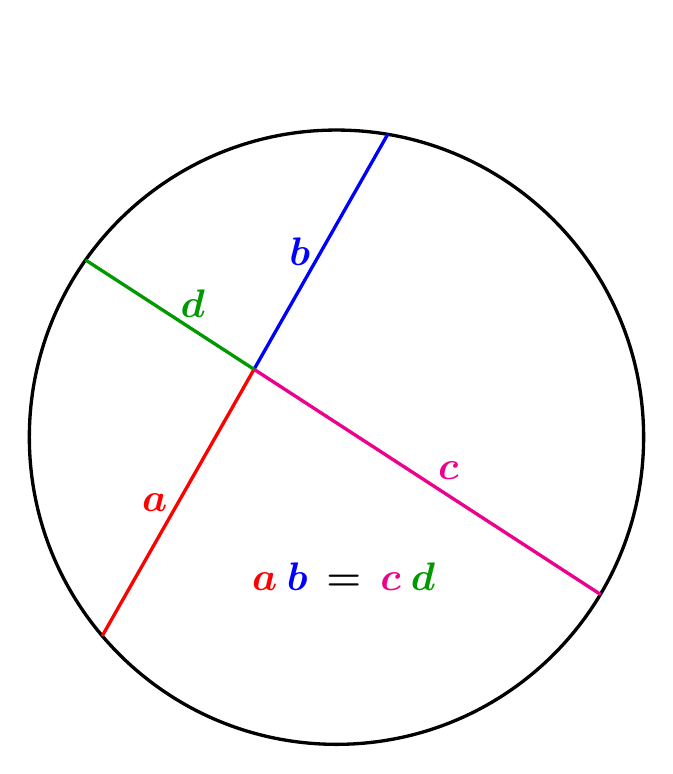
\begin{tikzpicture}[scale=1.3]
% Circle goes from (a) to (b)
\coordinate (a) at (0,0);
\coordinate (b) at (6,0);
% Line containing lower points is (c) -- (d)
\coordinate (c) at (0,-2);
\coordinate (d) at (6,-1.5);
% Line containing upper points is (e) -- (f)
\coordinate (e) at (0,1.5);
\coordinate (f) at (6,4);
% Name the upper and lower lines
\path [name path=chord1] (c) -- (d);
\path [name path=chord2] (e) -- (f);
% Draw a circle whose center is half-way between (a) and (b) through (a)
\node [draw,very thick,circle through=(a),name path=circ] at ($ (a)!.5!(b) $) {};
% Get intersections of the upper and lower lines with the circle
\path [name intersections={of=circ and chord1,by={i1,i2}}];
\path [name intersections={of=circ and chord2,by={i3,i4}}];
% Name the two chords
\path [name path=x1] (i1) -- (i3);
\path [name path=x2] (i2) -- (i4);
% Get their intersection
\path [name intersections={of=x1 and x2,by={p}}];
% Draw four lines from intersection to circle
\draw[very thick,red] (i1) -- node[left] {\mth{a}} (p);
\draw[very thick,blue] (p) --  node[left] {\mth{b}} (i3);
\draw[very thick,magenta] (i2) -- node[right,yshift=4pt] {\mth{c}} (p);
\draw[very thick,green!60!black] (p) -- node[right,yshift=4pt] {\mth{d}} (i4);
% Display formula in color
\begin{scope}[xshift=2.3cm,yshift=-1.5cm]
\node[anchor=base,red] at (0,0) {\mth{a}};
\node[anchor=base,blue] at (9pt,0) {\mth{b}};
\node[anchor=base] at (22pt,0) {\mth{=}};
\node[anchor=base,magenta] at (35pt,0) {\mth{c}};
\node[anchor=base,green!60!black] at (44pt,0) {\mth{d}};
\end{scope}
\end{tikzpicture}
%
\hspace{40mm}
%
% Intersecting secants
%
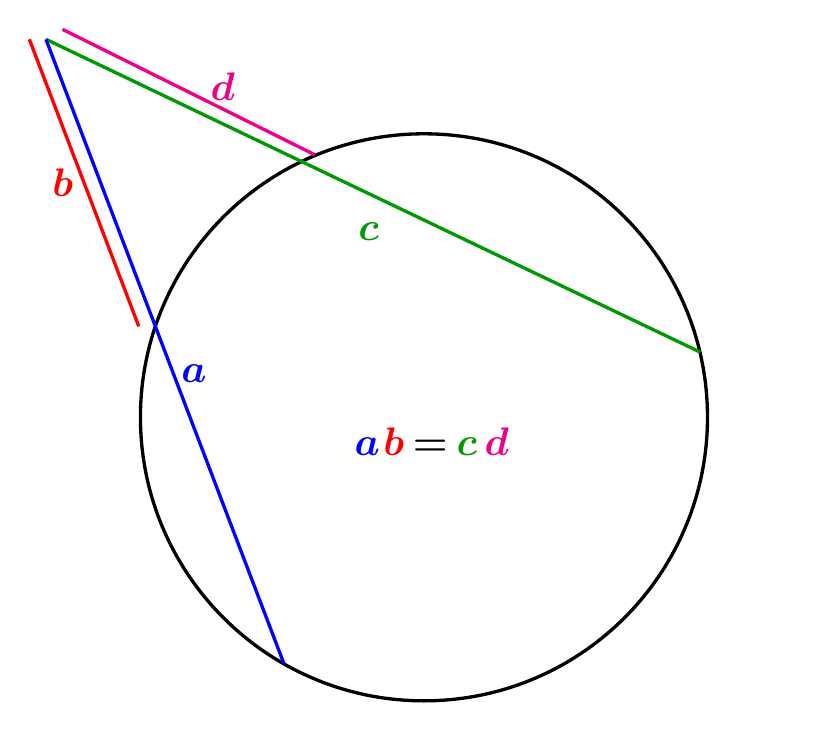
\begin{tikzpicture}[scale=1.2]
% Circle goes from (a) to (b)
\coordinate (a) at (0,0);
\coordinate (b) at (6,0);
% Line containing lower points is (c) -- (d)
\coordinate (c) at (1,-3);
\coordinate (d) at (7,1.5);
% Point outside circle is (e)
\coordinate (e) at (-1,4);
% Name the lower chord
\path [name path=chord] (c) -- (d);
% Draw a circle whose center is half-way between (a) and (b) through (a)
\node [draw,very thick,circle through=(a),name path=circ] at ($ (a)!.5!(b) $) {};
% Get intersection of the lower line with the circle
\path [name intersections={of=circ and chord,by={i1,i2}}];
% Draw the full secants
\draw [name path=secant1,very thick,green!60!black] (i1) -- node[left,xshift=6pt,yshift=-13pt] {\mth{c}} (e);
\draw [name path=secant2,very thick,blue] (i2) -- node[right,xshift=2pt,yshift=-8pt] {\mth{a}} (e);
% Get intersections of the secants with the circle
\path [name intersections={of=circ and secant1,by={s11,s12}}];
\path [name intersections={of=circ and secant2,by={s21,s22}}];
% Draw offset lines from outside point
%   with the intersections of the secants
\draw[very thick,red]
  let \p1 = (s21), \p2 = (e) in
    (\x2-5pt,\y2) -- node[left] {\mth{b}} (\x1-5pt,\y1);
\draw[very thick,magenta]
  let \p1 = (s12), \p2 = (e) in
    (\x2+5pt,\y2+3pt) -- node[right,xshift=4pt,yshift=2pt] {\mth{d}} (\x1+4pt,\y1+2pt);
% Display formula in color
\begin{scope}[xshift=2.4cm,yshift=-4mm]
\node[anchor=base,blue] at (0,0) {\mth{a}};
\node[anchor=base,red] at (8pt,0) {\mth{b}};
\node[anchor=base] at (19pt,0) {\mth{=}};
\node[anchor=base,green!60!black] at (30pt,0) {\mth{c}};
\node[anchor=base,magenta] at (39pt,0) {\mth{d}};
\end{scope}
\end{tikzpicture}
%
\hspace{30mm}
%
% Intersecting tangent and secant
%
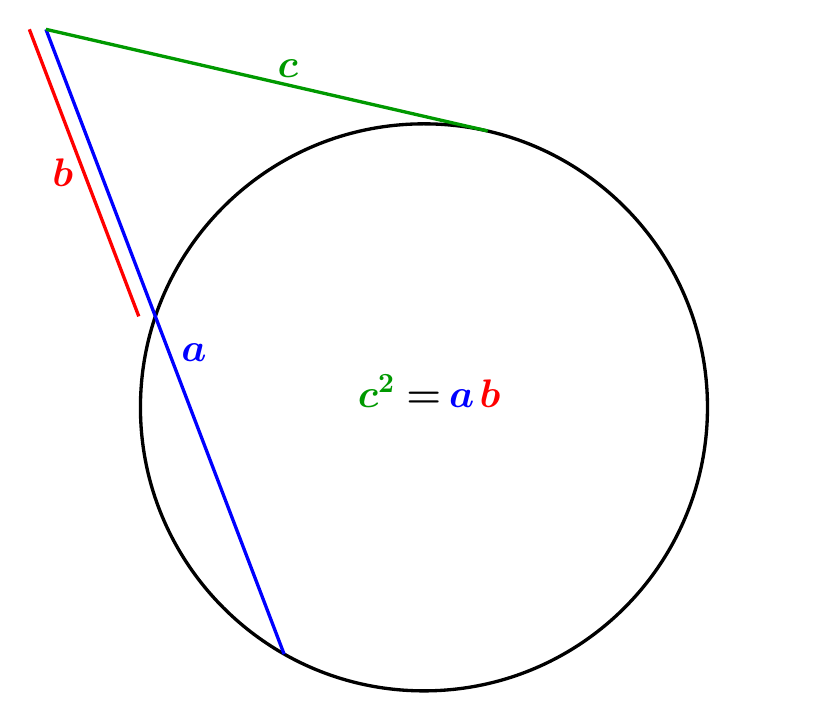
\begin{tikzpicture}[scale=1.2]
% Circle goes from (a) to (b)
\coordinate (a) at (0,0);
\coordinate (b) at (6,0);
% Line containing lower points is (c) -- (d)
\coordinate (c) at (1,-3);
\coordinate (d) at (7,1.5);
% Point outside circle is (e)
\coordinate (e) at (-1,4);
% Name the lower chord
\path [name path=chord] (c) -- (d);
% Draw a circle whose center is half-way between (a) and (b) through (a)
\node [draw,very thick,circle through=(a),name path=circ] (circle) at ($ (a)!.5!(b) $) {};
% Get intersection of the lower line with the circle
\path [name intersections={of=circ and chord,by={i1,i2}}];
% Draw the full secant
\draw [name path=secant2,very thick,blue] (i2) -- node[right,yshift=-4pt,xshift=2pt] {\mth{a}} (e);
% Get intersection of the secant with the circle
\path [name intersections={of=circ and secant2,by={s21,s22}}];
% Draw offset line from outside point
%   with the intersection of the secant
\draw[very thick,red]
  let \p1 = (s21), \p2 = (e) in
    (\x2-5pt,\y2) -- node[left] {\mth{b}} (\x1-5pt,\y1);
% Draw the tangent line
\coordinate (tan) at (tangent cs:node=circle, point={(e)}, solution=2);
\draw[very thick,green!60!black] (e) -- node[right,yshift=4pt] {\mth{c}} (tan);
% Display formula in color
\begin{scope}[xshift=2.5cm]
\node[anchor=base,green!60!black] at (0,0) {\mth{c^2}};
\node[anchor=base] at (.5,0) {\mth{=}};
\node[anchor=base,blue] at (.9,0) {\mth{a}};
\node[anchor=base,red] at (1.2,0) {\mth{b}};
\end{scope}
\end{tikzpicture}
\end{center}
\end{document}
